% In Latex the % symbol will indicate a comment. Text following the % symbol will not appear in the generated document and allow you to annotate your latex file
% This document is a modified version of the "sample document" provided by the American Journal of Physics through their author's guide.

\documentclass[prl,twocolumn]{revtex4-1}  % The "prl" tells latex to use the physical review letters formatting with one column from the revtex4.1 document class
%\documentclass[prl,preprint,linenumbers]{revtex4-1}  % other options can change formatting for various purposes. For example you can include line numbers with "linenumbers" and the "preprint" to make things easier to edit. Similarly you could use "singlecolumn" and "doublespace"
% NOTE: only a single documentclass should be declared. Comment out the other one. You can try changing styles and classes and compiling the document to see one of the benefits of Latex, the ease of reformatting.
\usepackage{chemformula}
\usepackage{color}
\usepackage{listings}
\usepackage{array, booktabs, makecell}
\usepackage{siunitx, mhchem}
\definecolor{dkgreen}{rgb}{0,0.6,0}
\definecolor{gray}{rgb}{0.5,0.5,0.5}
\definecolor{mauve}{rgb}{0.58,0,0.82}
\usepackage{float}
\usepackage{physics}
\definecolor{codegreen}{rgb}{0,0.6,0}
\definecolor{codegray}{rgb}{0.5,0.5,0.5}
\definecolor{codepurple}{rgb}{0.58,0,0.82}
\definecolor{backcolour}{rgb}{0.95,0.95,0.92}
 \definecolor{mygreen}{RGB}{28,172,0} % color values Red, Green, Blue
\definecolor{mylilas}{RGB}{170,55,241}
\usepackage{color}
\usepackage{listings}
 \lstset{language=Matlab,%
    %basicstyle=\color{red},
    breaklines=true,%
    morekeywords={matlab2tikz},
    keywordstyle=\color{blue},%
    morekeywords=[2]{1}, keywordstyle=[2]{\color{black}},
    identifierstyle=\color{black},%
    stringstyle=\color{mylilas},
    commentstyle=\color{mygreen},%
    showstringspaces=false,%without this there will be a symbol in the places where there is a space
    numbers=left,%
    numberstyle={\tiny \color{black}},% size of the numbers
    numbersep=9pt, % this defines how far the numbers are from the text
    emph=[1]{for,end,break},emphstyle=[1]\color{red}, %some words to emphasise
    %emph=[2]{word1,word2}, emphstyle=[2]{style},    
}
 



\usepackage{amsmath}  % needed for \tfrac, \bmatrix, etc.
\usepackage{amsfonts} % needed for bold Greek, Fraktur, and blackboard bold
\usepackage{graphicx} % needed for figures
\usepackage{hyperref} % needed for clickable links
\usepackage{lipsum} 
\newcommand{\term}[0]{Fall 2018} 

\begin{document}

% Be sure to use the \title, \author, \affiliation, and \abstract macros
% to format your title page.  Don't use lower-level macros to  manually
% adjust the fonts and centering.

\title{ Stat-Mech Paper }
% In a long title you can use \\ to force a line break at a certain location.
\author{Leticia Damian }
\email{Damia005@cougars.csusm.edu}
\author{Joshua Lucas}
\email{Lucas035@cougars.csusm.edu}
\author{Rowan Ranjbar}
\email{ranjb001@cougars.csusm.edu}


% optional
% If there were a second author at the same address, we would put another 
% \author{} statement here.  Don't combine multiple authors in a single
% \author statement.
% Please provide a full mailing address here.
\affiliation{Department of Physics, California State University San Marcos, San Marcos, CA 92096}



% See the REVTeX documentation for more examples of author and affiliation lists.
% or google

%\date{\today}

\begin{abstract}

\end{abstract}
 

\maketitle % title page is now complete

\section{Introduction}

While the polar axis of earth is tilted on its axis by $23.5^{\circ}$ from the elliptic plane the moon, even tilted $5^{\circ}$ on its orbit plane, i inclined by only $1.5^{\circ}$ on its polar axis\citep{Koebel}. This means that locations at the lunar poles are horizontal to the light from the sun. 

\section{Habitat Location}
The loation of the habitat requires at least four basic requirments, proximaty to water, communication line-of-sight with Earth, illumination , and traversable terrain. It is the intersection of these componets where we find the most habital location to be the southern lunar pole.


\section{Illumination Info}


\begin{figure}[!h]
\centering
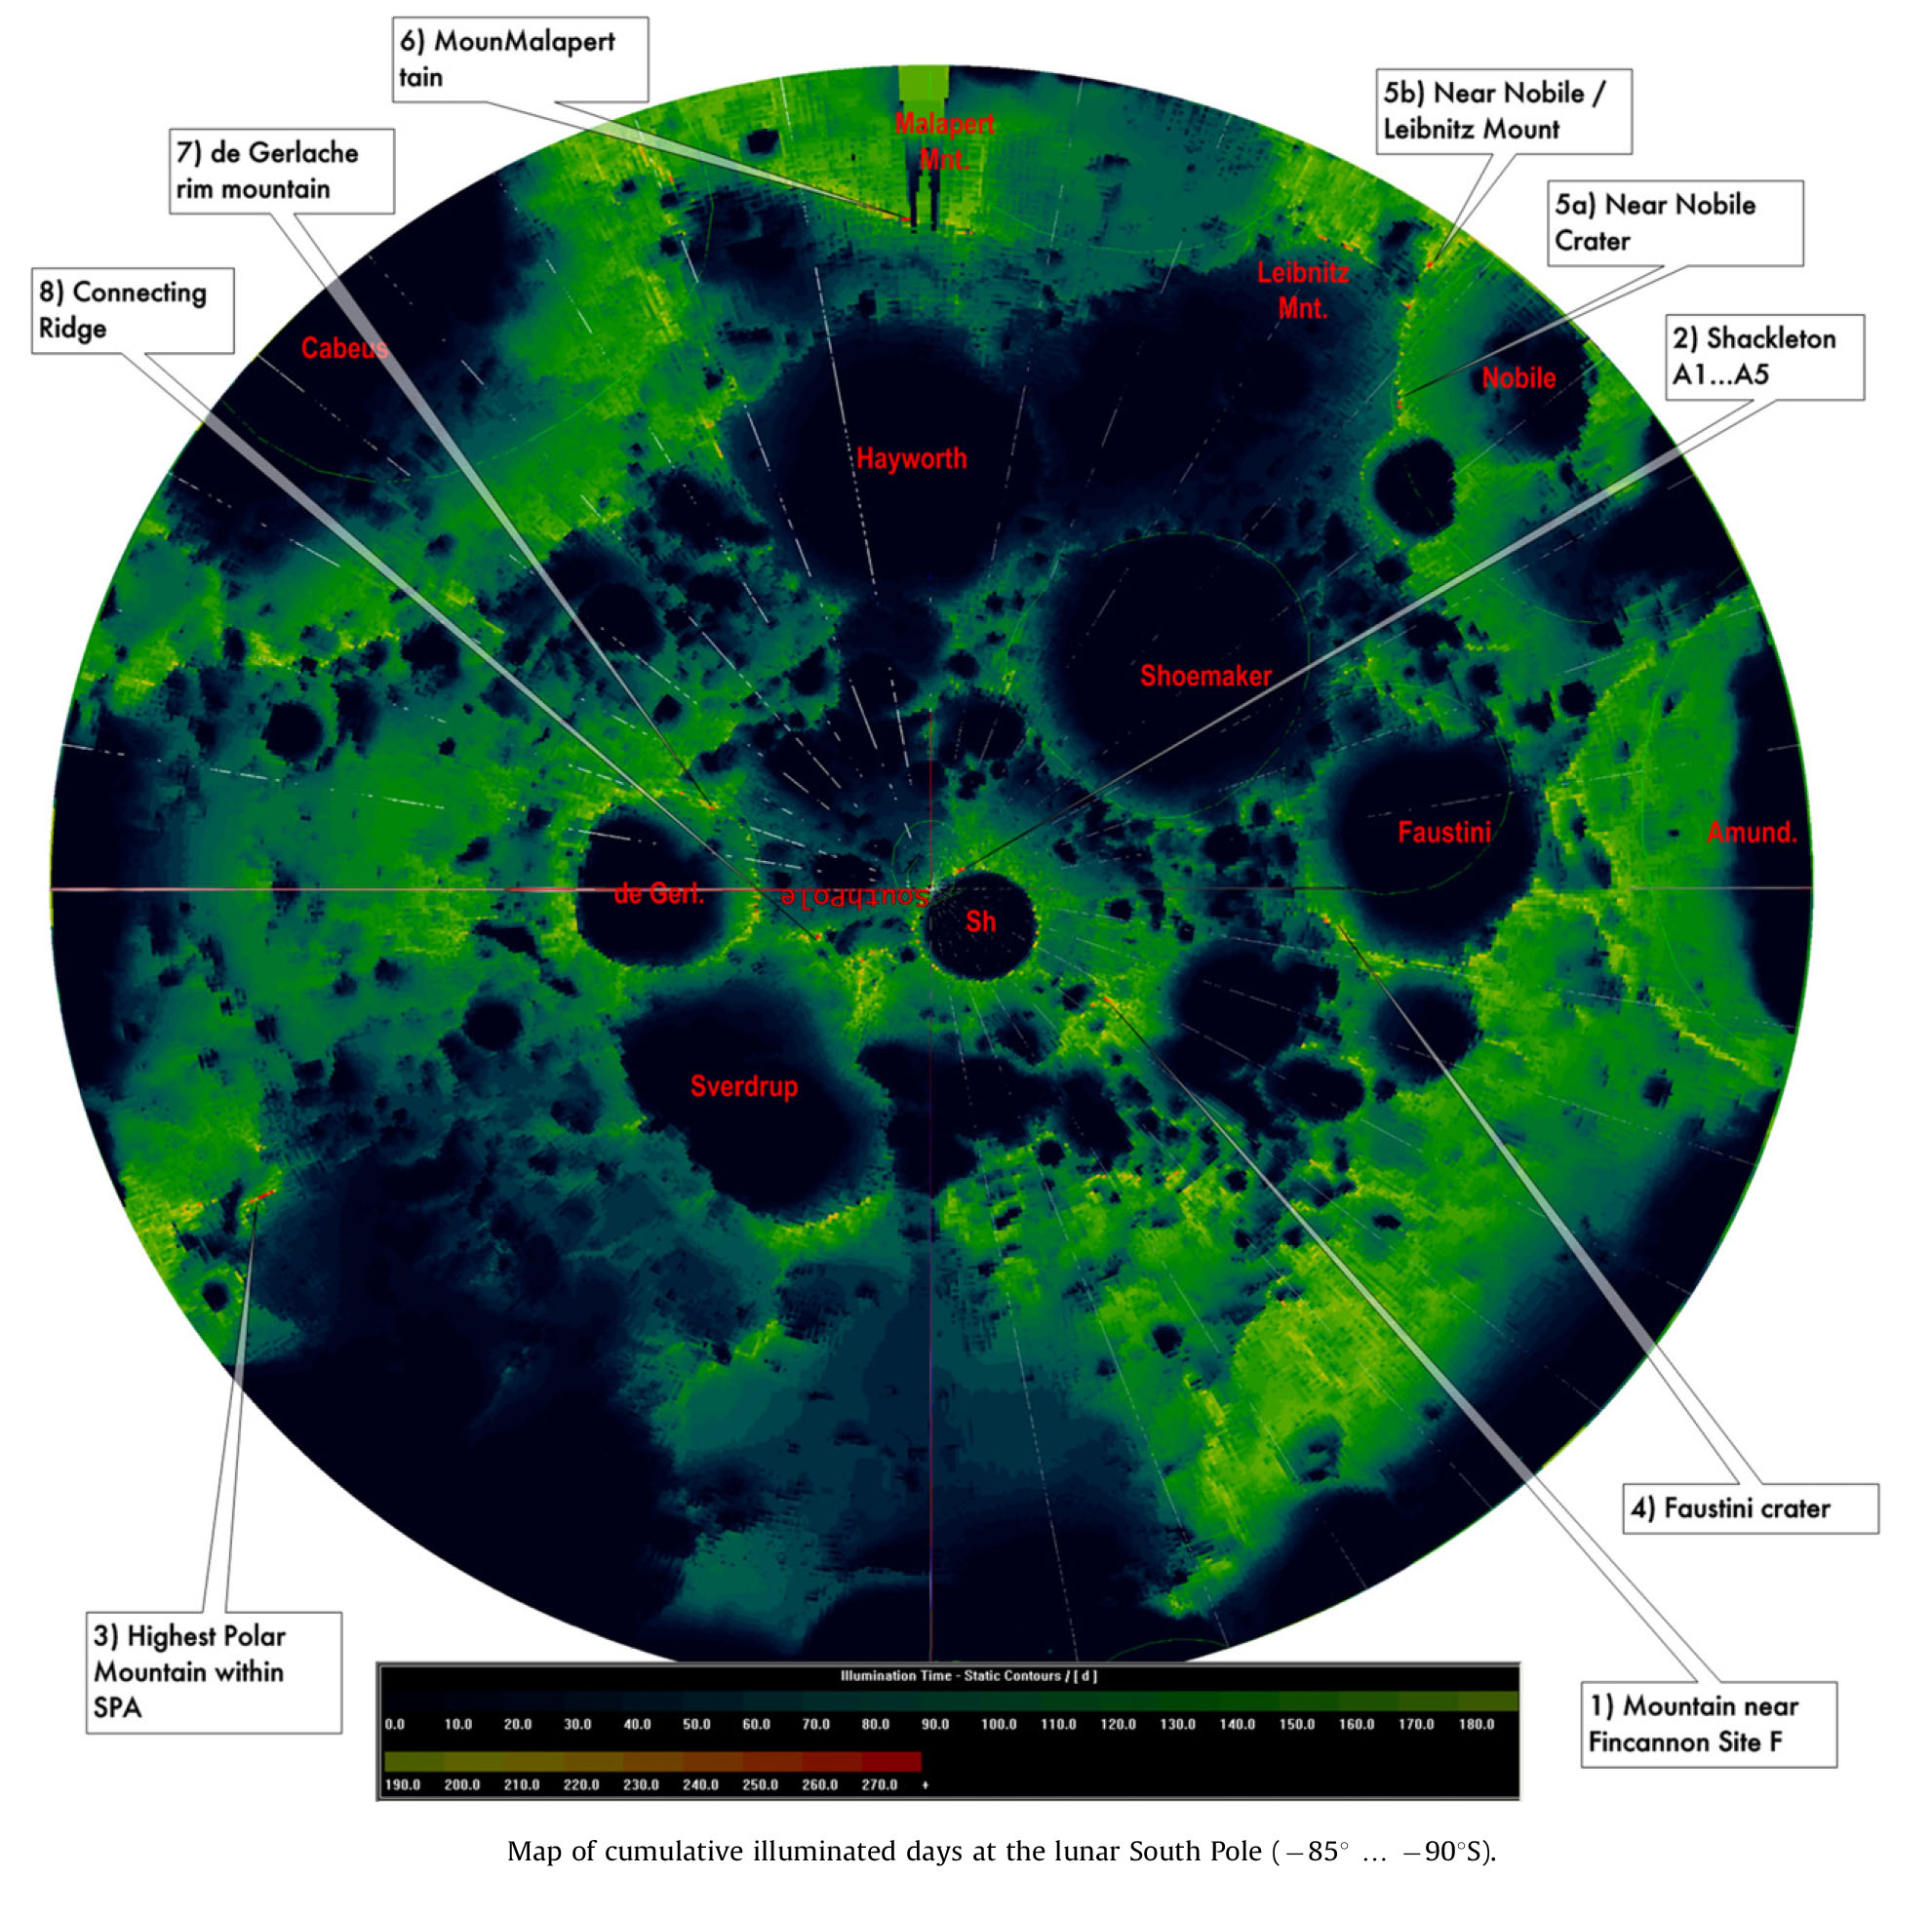
\includegraphics[width = \linewidth]{South_Pole_Light.jpg}
\caption{ The Gaussian distribution of the data. }
\end{figure}

``The solar elevation is dependent upon the lunar seasons, with solstices of $-1.54^{\circ}$ during lunar winter,and $+1.54^{\circ}$ during lunar summer. There thus exist mountain peaks that are characterized by near eternal illumination, which provide a benign thermal environment for any long-term robotic or manned lander mission and ideal conditions for photovoltaic power generation. Sunlit polar surfaces feature moderate temperature variations of $10^{\circ} \pm 50^{\circ}C$ [2]''\citep{Koebel}.

``In contrast to this,depressed polar surfaces,like crater grounds,lie in near permanent darkness, and are thus very cold. Uncertainties in lunar heat flow values [3] suggest that the temperatures within these cold traps vary between 50 and 70K. At these temperatures, atoms and molecules of volatile species cannot escape [4]. The smaller impact
craters in the polar region are therefore believed to harbour
water resources that remain conserved through the cryogenic temperatures inside them.''\citep{Koebel}


\section{Generating Power}

\section{Regolith Usage}

\section{Regolith Thermal Properties}


\begin{figure}[!h]
\centering
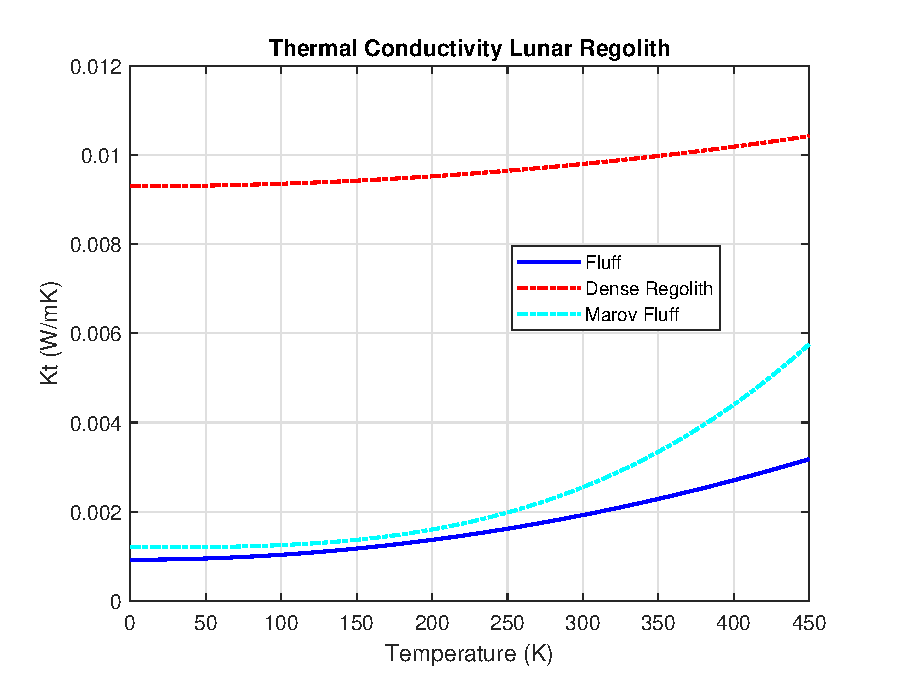
\includegraphics[width = \linewidth]{thermal_conductivity.eps}
\caption{ The Gaussian distribution of the data. }
\end{figure}


\begin{figure}[!h]
\centering
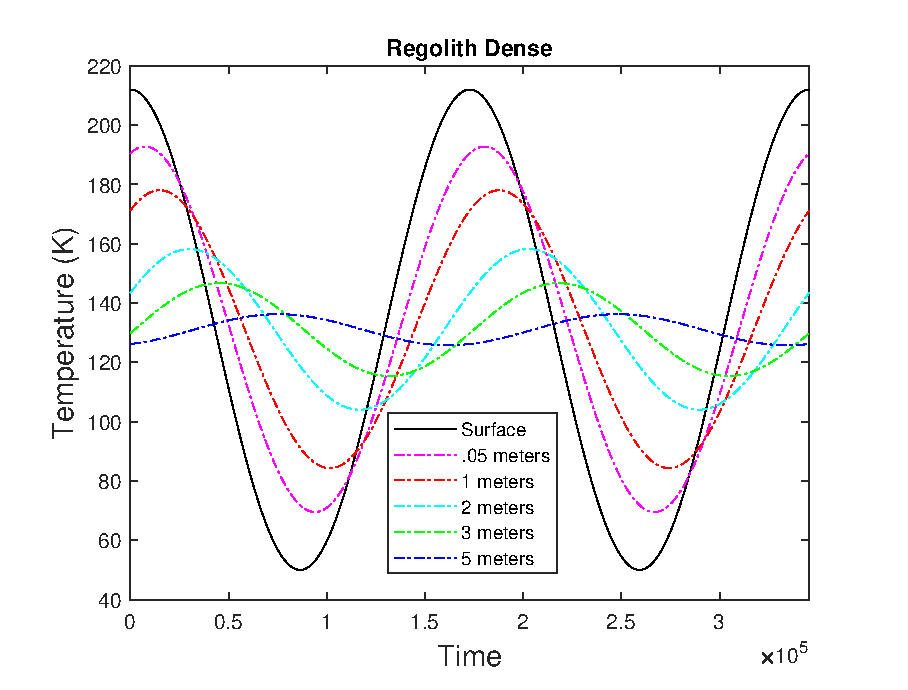
\includegraphics[width = \linewidth]{Regolith_Pulse.eps}
\caption{ The Gaussian distribution of the data. }
\end{figure}


\begin{figure}[!h]
\centering
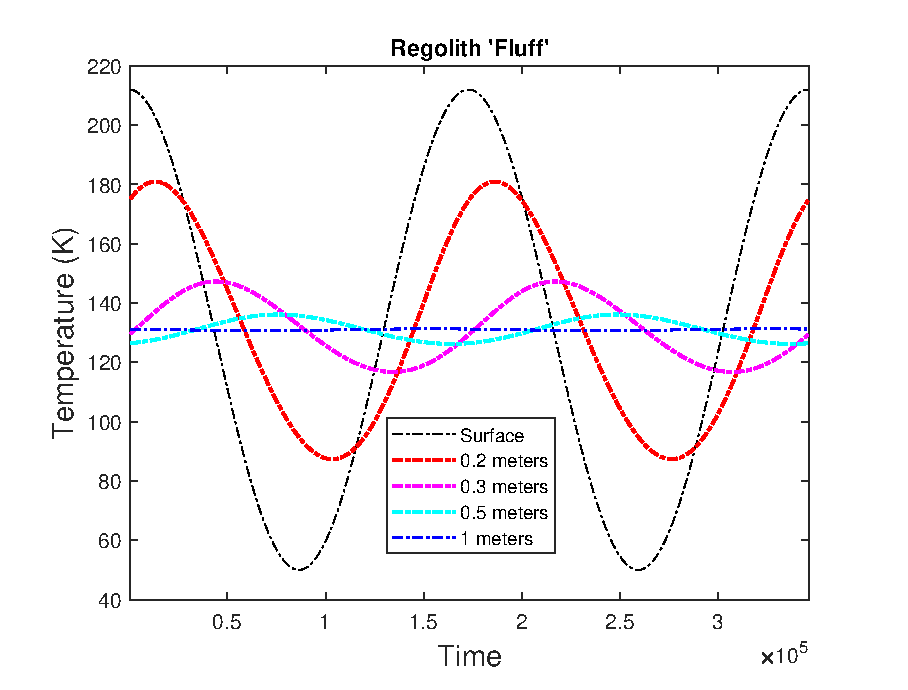
\includegraphics[width = \linewidth]{Processed_Regolith.eps}
\caption{ The Gaussian distribution of the data. }
\end{figure}
\section{Habitat thermal}

\begin{figure}[!h]
\centering
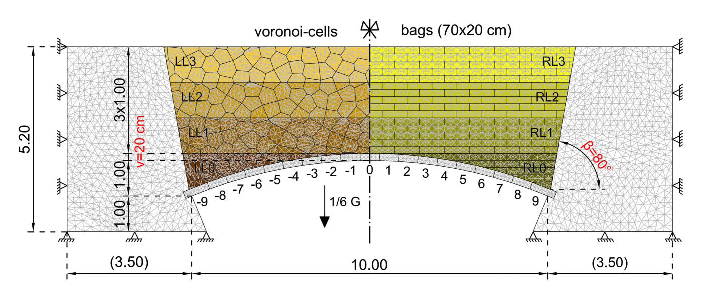
\includegraphics[width = \linewidth]{bags.eps}
\caption{ The Gaussian distribution of the data. }
\end{figure}



\section{Conclusion}

\appendix*   % Omit the * if there's more than one appendix.


\section{ Acknowledgments}

 All figures were created in Matlab and the paper was typeset in \LaTeX.
\begin{acknowledgments}


\end{acknowledgments}

\begin{thebibliography}{99}
% The numeral (here 99) in curly braces is nominally the number of entries in
% the bibliography. It's supposed to affect the amount of space around the
% numerical labels, so only the number of digits should matter--and even that
% seems to make no discernible difference.

\bibitem{Koebel}David Koebel, Michele Bonerba, Daniel Behrenwaldt, Matthias Wieser, Carsten Borowy,
Analysis of landing site attributes for future missions targeting the rim of the lunar South Pole Aitken basin,
Acta Astronautica,
Volume 80,
2012,
Pages 197-215



\end{thebibliography}

\end{document}
